\documentclass[11pt,a4paper]{article}

% Shared preamble for the EM-LLM Reader's Companion.
% Loaded once from main.tex; chapters never repeat \usepackage.

\usepackage[utf8]{inputenc}
\usepackage[T1]{fontenc}
\usepackage{lmodern}
\usepackage[a4paper,margin=1in]{geometry}
\usepackage{microtype}

\usepackage{amsmath}
\usepackage{amssymb}
\usepackage{amsthm}
\usepackage[ruled,linesnumbered]{algorithm2e}
\usepackage{array}
\usepackage{booktabs}
\usepackage{seqsplit}
\usepackage{xcolor}
\usepackage{enumitem}
\usepackage{csquotes}

\usepackage{listings}
\usepackage{tikz}
\usetikzlibrary{positioning,arrows.meta,calc,fit,backgrounds,decorations.pathreplacing,shapes.geometric}

\usepackage[backend=biber,style=numeric,sorting=none,maxbibnames=99]{biblatex}
\addbibresource{refs.bib}

\usepackage[colorlinks=true,linkcolor=black!70!blue,citecolor=black!50!blue,urlcolor=black!50!blue]{hyperref}
\usepackage[capitalize,noabbrev]{cleveref}

% Python listing style. The intent here is dense but readable code on the page,
% so we keep numbers on the left and avoid heavy frames that fight with the
% body text.
\definecolor{lstbg}{HTML}{F7F7F2}
\definecolor{lstkw}{HTML}{0B4F6C}
\definecolor{lststr}{HTML}{8B5E00}
\definecolor{lstcom}{HTML}{577590}

\lstdefinestyle{pythonstyle}{
    language=Python,
    backgroundcolor=\color{lstbg},
    basicstyle=\ttfamily\footnotesize,
    keywordstyle=\color{lstkw}\bfseries,
    stringstyle=\color{lststr},
    commentstyle=\color{lstcom}\itshape,
    numbers=left,
    numberstyle=\tiny\color{black!50},
    numbersep=8pt,
    showstringspaces=false,
    breaklines=true,
    breakatwhitespace=true,
    tabsize=4,
    frame=single,
    framerule=0.3pt,
    rulecolor=\color{black!30},
    captionpos=b,
    xleftmargin=10pt,
    xrightmargin=4pt,
    aboveskip=0.6em,
    belowskip=0.6em,
}
\lstset{style=pythonstyle}

% Shell snippets reuse the same frame but keep the default lexer.
\lstdefinestyle{shellstyle}{
    language=bash,
    backgroundcolor=\color{lstbg},
    basicstyle=\ttfamily\footnotesize,
    keywordstyle=\color{lstkw}\bfseries,
    commentstyle=\color{lstcom}\itshape,
    numbers=none,
    showstringspaces=false,
    breaklines=true,
    frame=single,
    framerule=0.3pt,
    rulecolor=\color{black!30},
    xleftmargin=10pt,
    xrightmargin=4pt,
}

% Convenience commands for frequently used objects.
% \seqsplit lets long identifiers and paths break across line ends without
% sliding into the right margin. Marked robust so the macros survive being
% used inside moving arguments (section titles, captions, TOC entries).
\DeclareRobustCommand{\file}[1]{\texttt{\seqsplit{#1}}}
\DeclareRobustCommand{\code}[1]{\texttt{\seqsplit{#1}}}
\newcommand{\param}[1]{\ensuremath{#1}}
\newcommand{\Surprise}{\mathcal{S}}
\newcommand{\Adj}{\mathbf{A}}
\newcommand{\Modularity}{Q}
\newcommand{\Conductance}{\phi}

\theoremstyle{definition}
\newtheorem{definition}{Definition}[section]
\newtheorem{example}{Example}[section]

\setlist{itemsep=2pt,topsep=4pt}


\title{An EM-LLM Reader's Companion\\[0.4em]
  \large Concepts, Code, and Reproduction Notes for the Fountas et al.\ (2025) Episodic Memory LLM}
\author{Juan Pablo Morande}
\date{\today}

\begin{document}
\maketitle

\begin{abstract}
\noindent
This companion walks through \emph{Human-Inspired Episodic Memory for Infinite Context LLMs} by \textcite{fountas2025emllm}, paired with a function-level guide to the implementation that ships with the paper and the wrappers that drive the NeurIPS 2026 MLRC reproduction in this repository. The first part rebuilds the paper's reasoning in plain language with worked examples, equations, and references back to specific paper sections. The second part traces the code path from token to attention output across \file{em\_llm/}, the benchmark harness, and the reproduction scripts. The document is meant to be read alongside the paper PDF and a code editor open on \file{em-llm-model/}, not as a replacement for either.
\end{abstract}

\tableofcontents
\newpage

\section*{Preface}
\addcontentsline{toc}{section}{Preface}

This document was written for one reader: someone sitting down to reproduce \textcite{fountas2025emllm} and wanting a single place that explains both the paper's machinery and the code that implements it. It assumes familiarity with transformer attention, with the basics of long-context inference, and with the conventions of a Hugging Face training stack. It does not assume prior exposure to event-cognition theory, graph-based clustering metrics, or the particular abstractions used inside \file{em\_llm/}.

The chapters are ordered to be read straight through, but each is intended to stand on its own when used as a reference. Part I covers the paper. Chapter~1 places the work in context and gives the headline results. Chapter~2 builds the cognitive-science background that makes the rest of the paper legible. Chapter~3 is the longest of Part I and steps through the three core innovations (surprise-based segmentation, graph-theoretic boundary refinement, two-stage retrieval) with worked examples. Chapters~4 and~5 cover architecture, hyperparameters, and the experimental setup. Chapter~6 closes Part I with limitations and open questions.

Part II is the code companion. Chapter~7 maps the repository so the reader knows what is vendored, what is reproduction-specific, and how OmegaConf layers configuration at runtime. Chapter~8 is the function-by-function walk through \file{em\_llm/}, which is where the paper's algorithm actually lives. Chapter~9 covers the benchmark harness, and Chapter~10 covers the reproduction scripts in \file{reproduction/}. Two appendices follow: a glossary for the cognitive-science and graph-theory vocabulary, and a notation table.

A note on the relationship between this document and the paper. Anywhere the explanation here improves on or diverges from the paper's phrasing, it is in service of the reader, not as a correction. Where the paper introduces a symbol, a section, a figure, or an algorithm, the companion references it explicitly so the reader can flip to the original. Where the code uses a name that differs from the paper, both names appear together the first time the concept is introduced.


\part{The paper}

\section{The paper at a glance}
\label{sec:paper-overview}

\subsection{Bibliographic data}
\label{sec:bib}

\emph{Human-Inspired Episodic Memory for Infinite Context LLMs} was published at ICLR 2025 by Zafeirios Fountas, Martin A.\ Benfeghoul, Adnan Oomerjee, Fenia Christopoulou, Gerasimos Lampouras, and Haitham Bou-Ammar (all Huawei Noah's Ark Lab, London), together with Jun Wang (AI Centre, UCL) \cite{fountas2025emllm}. Benfeghoul and Oomerjee are listed as equal contributors. The companion code is at \url{https://github.com/em-llm/EM-LLM-model}, and the reproduction in this repository pins commit \texttt{edb2e4a} of that codebase under \file{em-llm-model/}.

The paper proposes EM-LLM, an inference-time wrapper that gives a pre-trained transformer access to context lengths far beyond its training window. It does so by carving the incoming token stream into episodic events, storing those events in a KV cache that can spill to CPU or disk, and pulling them back in through a two-stage retrieval process whenever the model needs to attend further than its local window allows. No fine-tuning is required; the underlying LLM weights stay frozen.

The headline experimental claims are three. First, EM-LLM outperforms InfLLM \cite{xiao2024infllm}, the previous state of the art in group-based KV retrieval, on LongBench \cite{bai2023longbench} and $\infty$-Bench \cite{zhang2024infbench} across five different base LLMs (Mistral-7B, LLaMA-2-7B, LLaMA-3-8B, LLaMA-3.1-8B, Phi-3, Phi-3.5). Second, it beats RAG with the NV-Embed-v2 retriever \cite{lee2024nvembed} by 30.5 points on LongBench and 11.5 on $\infty$-Bench when run on LLaMA-3.1-8B. Third, the system retrieves correctly on a passkey task with sequences up to 10.2 million tokens, a length at which full-attention baselines are computationally out of reach \cite{ding2024longrope}.

\subsection{One-page plain-English summary}
\label{sec:summary}

The starting observation is cognitive. Humans do not store experience as a flat sequence of moments; we segment it into events, and the boundaries between events line up with moments of high prediction error. Once the brain has chopped experience into events, recall is driven by similarity to the present query and by the temporal neighbourhood of whatever event we have just remembered. EM-LLM imports these two ingredients into a transformer.

For event segmentation, the paper repurposes the LLM's own next-token surprise as a boundary signal. The surprise at position $t$ is $-\log P(x_t \mid x_{<t}; \theta)$, a quantity the model computes anyway. Tokens whose surprise exceeds a moving threshold $T_t = \mu_{t-\tau:t} + \gamma \, \sigma_{t-\tau:t}$ are treated as candidate event boundaries (Eq.\ 1 of the paper). The threshold tracks local statistics so that a passage of unusually predictable or unusually noisy text does not over- or under-segment. A second pass then refines these boundaries by walking the similarity matrix of attention keys within the local window: each candidate boundary is moved to the position that maximises modularity or minimises conductance of the induced graph, the same metrics used for community detection in network science.

For memory retrieval, each layer holds two buffers. A \emph{similarity buffer} of $k_s$ events is filled by a $k$-NN lookup over event representatives, chosen as the most influential tokens within each event in the sense of \textcite{xiao2024infllm}. A \emph{contiguity buffer} of $k_c$ events holds the temporal neighbours of whatever events were just retrieved, mimicking the contiguity effect in human free recall \cite{howard2002contiguity}. The two buffers together, alongside an attention-sink prefix of 128 initial tokens \cite{xiao2024attsinks} and the local context window, make up the LLM's effective context at each layer. Crucially, every layer retrieves independently, so different layers can focus on different parts of the history.

The training-free property is what makes the method practical. Surprise is read off the existing forward pass. The refinement step costs $O(nm)$ for sequence length $n$ and chunk size $m$. The $k$-NN can be exact for small memories and approximate (FAISS-style) at scale. None of this requires touching the LLM weights or its tokenizer.

Where this matters in numbers: on Mistral-v0.2, surprise plus refinement plus contiguity buffer (\emph{SM+C}) lifts the LongBench retrieval-task score from 64 to 84.1 over InfLLM at the same context budget, while edging the overall LongBench average from 41.9 to 43.7 (paper Table~1). On LLaMA-3.1-8B the gains are smaller in aggregate (51.1 to 51.3), but the $\infty$-Bench Retrieve.KV score moves from 81 to 90.2. The 10M-token passkey claim is the single most striking result: every other system in the comparison saturates well below 10M tokens, and EM-LLM holds 100\% accuracy at that scale (paper Fig.~1).

\subsection{Place in the long-context literature}
\label{sec:literature}

EM-LLM lives in the retrieval-based corner of long-context work, not in the architecture-modification corner. There is a long line of papers that try to extend context by changing positional encodings (linear scaling, NTK scaling, YaRN, LongRoPE) or by training on longer sequences with budget-aware attention (LongLoRA, LongRoPE-2048k). EM-LLM does none of that; the base LLM is unchanged.

The most direct ancestor is the group-based $k$-NN retrieval line. Memorizing Transformers \cite{wu2022memorizing} and the Focused Transformer \cite{tworkowski2023focused} fetched individual KV pairs from external memory. InfLLM \cite{xiao2024infllm} moved to fetching contiguous blocks instead of individual tokens, which is closer to how humans recall scenes rather than instants. EM-LLM keeps the block-fetch idea but replaces InfLLM's fixed-size segmentation with one driven by the LLM's own surprise signal, then refines block boundaries with graph metrics. This is the precise contribution: not a new retrieval algorithm, but a more adaptive way of deciding what counts as a block in the first place, plus a second buffer for temporal neighbours.

EM-LLM also competes with RAG-style systems, where retrieval happens once at the prompt level using a separate embedding model such as NV-Embed-v2 \cite{lee2024nvembed}. The relevant difference is granularity: RAG attends to retrieved chunks once, at the input layer; EM-LLM attends per layer, so different attention heads can pull in different events. The paper attributes much of its margin over RAG (Fig.~1, Section~4.1) to this layer-wise property rather than to better retrieval per se.

The cognitive-science citations matter for reading the paper but are not load-bearing for the engineering. The brain-inspired framing is genuine, not decorative: surprise-as-boundary comes from \textcite{zacks2007event}, the contiguity buffer is grounded in \textcite{howard2002contiguity}, and the attention-sink prefix from \textcite{xiao2024attsinks} maps onto the working-memory analogy the authors invoke. Chapter~\ref{sec:background} unpacks these references; the rest of Part~I treats them as given.

There is one experimental claim that does not fit cleanly into the long-context bucket and is worth flagging here: the paper shows that surprise-only segmentation in an LLM correlates with human-annotated event boundaries on podcast transcripts (Section~4.2, Fig.~4). That result is a side observation in the paper, but it is the part most likely to interest readers from cognitive neuroscience, and it generalises the appeal of the work beyond NLP benchmarks.


\section{Background and problem statement}
\label{sec:background}

This chapter establishes the two intellectual halves the rest of the paper rests on. The first is the machine-learning side: why long-context transformers are difficult, and which strands of prior work EM-LLM borrows from. The second is the cognitive-science side: a compact tour of the human-memory ideas the authors translate into algorithms. Readers comfortable with either half can skim it and pick the rest up in context.

\subsection{Why long context is hard}
\label{sec:why-long-context}

There are three concrete obstacles that recur across the long-context literature, and each maps onto a design choice EM-LLM makes later.

The first obstacle is positional encoding. Transformer attention has no built-in notion of order, so positions are injected through additive embeddings (the original setup of \textcite{vaswani2017attention}), through relative-position biases, or through rotational encodings like RoPE. The trouble is that none of these schemes extrapolate gracefully past the lengths seen at training time. \textcite{kazemnejad2024impact} compare the dominant variants and show that out-of-distribution position indices degrade attention quality even when the model has the FLOPs to process the longer input. EM-LLM sidesteps this by assigning retrieved tokens a fixed position embedding, following the approach of \textcite{xiao2024infllm}, rather than asking the LLM to reason about positions tens of millions of tokens deep.

The second obstacle is computational cost. Softmax attention is quadratic in sequence length, which makes brute-force long-context inference impractical past roughly $10^5$ tokens on commodity hardware. The paper does not try to speed up the underlying attention; it instead changes what gets attended to. The local window is processed with full softmax, and everything older is summarised into events that are paged in selectively. The effective per-step cost is dominated by the size of the local window plus the size of the retrieved buffer, not by the total sequence length.

The third obstacle is more subtle and motivates the cognitive framing. When a query attends over a long context, the resulting weighted sum of value vectors becomes a low-distinctiveness average. The longer the window, the more values get summed, and the more the output looks like an undifferentiated mean. \textcite{liu2024lostmiddle} document this effect empirically as the lost-in-the-middle pattern: performance is higher when the relevant information sits at the beginning or end of the context than when it sits in the middle. EM-LLM's response is to never attend to all of history at once. Each layer attends to the local window plus a small number of retrieved events, and the rest is invisible to the softmax for that step.

\subsection{Episodic memory in the human brain}
\label{sec:episodic}

The cognitive-science vocabulary in the paper is consistent across a handful of foundational references. The shortest path through them runs as follows.

\paragraph{Episodic versus semantic memory.}
\textcite{tulving1972episodic} drew the distinction that gives the paper its name. Episodic memory holds particular experiences anchored in time and place. Semantic memory holds generalised knowledge stripped of those anchors. A transformer's parameters are best read as semantic memory: facts and patterns abstracted away from any specific training example. EM-LLM adds a temporary episodic store on top, so that a long-context interaction can be treated as a stream of personal experiences the model can refer back to without changing its weights.

\paragraph{Bayesian surprise as an event signal.}
The mechanism the brain uses to chunk continuous experience into discrete events is not yet settled, but one durable proposal is that event boundaries fall at moments of high prediction error: the brain has a generative model of what should come next, and surprising input gets flagged as the start of something new \cite{zacks2007event}. \textcite{itti2009bayesian} formalised this idea by measuring surprise as the Kullback--Leibler divergence between the observer's prior and posterior beliefs, showing that this Bayesian definition predicts where humans actually look in natural images. \textcite{kumar2023neural} took the next step in the LLM setting, showing that an LLM's own next-token surprise on a podcast transcript lines up with where human listeners report the story shifting. EM-LLM picks up directly from this last result: the surprise it uses is exactly the negative log-likelihood that the base LLM already computes during inference.

\paragraph{Free recall and the contiguity effect.}
Human free recall is not a random walk through memory. \textcite{kahana1996contiguity} and the longer analysis by \textcite{howard2002contiguity} establish two robust regularities. First, items studied close together in time tend to be recalled close together (contiguity). Second, after recalling an item, the next item recalled is more often the one that originally followed it than the one that preceded it (forward asymmetry). These patterns hold across many list-learning paradigms and motivate EM-LLM's second retrieval buffer: when an event is fetched by similarity, its temporal neighbours are also brought into the context window so that the LLM can exploit any sequential structure those neighbours carry.

\paragraph{Working memory and attention sinks.}
\textcite{baddeley1992working} and \textcite{cowan2001focus} describe working memory as a small, attention-controlled subset of long-term memory that is held in active form to support the current task. In EM-LLM's architecture, the local context window plays that role: a few thousand recent tokens get the full softmax treatment, while everything older sits in episodic memory and is pulled in on demand. The 128 initial tokens at the start of the context behave differently, acting as attention sinks that stabilise the attention distribution in streaming inference \cite{xiao2024attsinks}. The cognitive analogy here is looser than the others; the authors are clear that the sinks are an engineering fix borrowed from prior work, not a cognitive postulate.

\subsection{From cognition to algorithm}
\label{sec:cognition-to-algorithm}

The translation from these cognitive ideas to EM-LLM's machinery is more literal than is usual in brain-inspired ML, and that is part of what makes the paper readable. Surprise-based segmentation becomes a thresholding rule on the LLM's own negative log-likelihood (Section~\ref{sec:method-segmentation}). Boundary refinement becomes a graph-clustering pass on the attention-key similarity matrix, using modularity or conductance to enforce intra-event coherence (Section~\ref{sec:method-refinement}). The contiguity effect becomes a queue of temporal neighbours that runs alongside the similarity-based retrieval (Section~\ref{sec:method-retrieval}). Working memory becomes the local context window, and the attention sinks at position zero handle a numerical stability problem the cognitive framing does not need to explain.

Each of these correspondences is a hypothesis the experiments then test. The agreement between LLM surprise and human-annotated event boundaries (Section~\ref{sec:human-alignment}) is the closest the paper gets to validating the cognitive framing on its own terms; everything else is judged on task performance.


\section{Method}
\label{sec:method}

The method has three moving parts and they can be read in order. First, the LLM's own surprise picks out candidate event boundaries (\cref{sec:method-segmentation}). Second, a graph-theoretic refinement step nudges those boundaries to positions that group similar keys together (\cref{sec:method-refinement}). Third, the events stored under the resulting segmentation are pulled back into the LLM's context through two complementary buffers (\cref{sec:method-retrieval}). Everything runs at inference time on a frozen base model.

\subsection{Event segmentation via Bayesian surprise}
\label{sec:method-segmentation}

The segmentation step asks a simple question of every token: did the model find this token unexpected? If yes, the token is a candidate event boundary. If no, the token continues the current event. The boundary detector is built on quantities the model already produces.

\paragraph{Surprise.}
For an autoregressive LLM with parameters $\theta$, the conditional probability $P(x_t \mid x_{<t}; \theta)$ is computed during the normal forward pass. The Bayesian surprise of the actually observed token $x_t$ is
\begin{equation}
  \Surprise(x_t) \;=\; -\log P(x_t \mid x_{<t}; \theta).
  \label{eq:surprise}
\end{equation}
This is the same quantity the cross-entropy loss is built on; the only twist is that EM-LLM uses it as a runtime feature rather than as a training signal.

\paragraph{Threshold rule.}
A token at position $t$ is treated as a candidate boundary when its surprise exceeds a moving threshold
\begin{equation}
  T_t \;=\; \mu_{t-\tau:t} \;+\; \gamma \, \sigma_{t-\tau:t},
  \label{eq:threshold}
\end{equation}
where $\mu_{t-\tau:t}$ and $\sigma_{t-\tau:t}$ are the running mean and standard deviation of $\Surprise$ over the trailing window of length $\tau$, and $\gamma$ is a fixed scaling constant. \cref{eq:threshold} is Eq.\ 1 of the paper. Two design choices are worth pulling out. First, $T_t$ adapts to the local distribution, which means a stretch of unusually predictable text (the middle of a procedural document, say) does not get over-segmented just because its absolute surprise is low. Second, $\gamma$ is the only knob a user typically tunes; the paper sweeps $\gamma \in \{1.0, 1.5, 2.0, 2.5, 3.0, 3.5\}$ and reports $\gamma = 1.0$ as the best default across all tested base models.

\paragraph{Worked example.}
Suppose the trailing window has mean surprise $\mu = 2.0$ and standard deviation $\sigma = 0.5$, and we use $\gamma = 1.0$. Then the threshold for the next token is $T = 2.0 + 1.0 \cdot 0.5 = 2.5$. Now imagine six consecutive surprises:
\begin{center}
\begin{tabular}{lcccccc}
  \toprule
  token index $t$    & 1   & 2   & 3   & 4   & 5   & 6 \\
  $\Surprise(x_t)$   & 1.9 & 2.4 & 3.1 & 2.0 & 1.8 & 2.7 \\
  boundary?          & no  & no  & yes & no  & no  & yes \\
  \bottomrule
\end{tabular}
\end{center}
Tokens 3 and 6 trip the threshold and enter the candidate boundary list $B$. Their surprise values are not the largest possible; what matters is that they exceed the local mean by more than $\gamma$ standard deviations. In a real run, $\mu$ and $\sigma$ themselves are updated as the window slides forward, so the threshold at token 6 reflects a different local distribution than the threshold at token 3.

\paragraph{Outputs of this step.}
After segmentation the system holds a list $B = (b_1, b_2, \dots, b_k)$ of candidate boundary positions. Each $b_i$ is a token index where $\Surprise$ exceeded the threshold. The interval $[b_i, b_{i+1})$ is a proposed event. These intervals are still provisional; the refinement step below moves the right edge of each interval to a nearby position that produces a more coherent group of keys.

\subsection{Boundary refinement via graph clustering}
\label{sec:method-refinement}

Surprise tells us \emph{where} the model was caught off guard. It does not, by itself, tell us where the cleanest split between two events lies. A high-surprise token might land a few positions before the actual semantic break, or a few positions after it. The refinement step closes that gap by looking at the similarity structure of the attention keys.

\paragraph{Similarity graph.}
For attention head $h$, the key vectors $K^h_1, \dots, K^h_n$ over the current local window can be assembled into a similarity matrix
\begin{equation}
  A^h_{ij} \;=\; \mathrm{sim}(K^h_i, K^h_j) \;=\; (K^h_i)^\top K^h_j,
  \label{eq:adjacency}
\end{equation}
which is Eq.\ 2 of the paper. The choice of dot product (rather than cosine or another distance) is deliberate: the same similarity drives the LLM's own attention scores, so optimising group structure under $A^h$ is more aligned with the model's downstream computation than optimising under a generic distance would be. Reading $A^h$ as the weighted adjacency matrix of a graph over tokens, the question becomes which partition of those tokens into contiguous segments forms the best community structure.

\paragraph{Modularity.}
Modularity is the network-science measure of how much more strongly connected nodes within a community are than would be expected by chance. For a partition with community labels $c_i$ and total edge weight $m = \sum_{ij} A^h_{ij}/2$,
\begin{equation}
  \Modularity(A^h, B) \;=\; \frac{1}{4m} \sum_{i,j} \left( A^h_{ij} - \frac{1}{2m} \sum_i A^h_{ij} \sum_j A^h_{ij} \right) \delta(c_i, c_j),
  \label{eq:modularity}
\end{equation}
where $\delta$ is the Kronecker delta (Eq.\ 3 of the paper). Higher modularity means edges concentrate inside communities. The refinement step seeks boundaries that maximise $\Modularity$.

\paragraph{Conductance.}
Conductance is the complementary measure. It looks at the fraction of total edge weight cut at a community boundary. For a candidate community $S \subset V$,
\begin{equation}
  \Conductance(A^h, B) \;=\; \min_{S \in V} \frac{\sum_{i \in S, j \notin S} A^h_{ij}}{\min(\mathrm{vol}(S), \mathrm{vol}(V \setminus S))},
  \label{eq:conductance}
\end{equation}
with $\mathrm{vol}(S) = \sum_{i,j \in S} A_{ij}$ (Eq.\ 4 of the paper). Lower conductance means the cut at the boundary is small relative to the internal density of either side. Refinement under conductance picks boundaries that minimise $\Conductance$.

\paragraph{The refinement algorithm.}
With either metric in hand, the algorithm walks the candidate boundary list and adjusts each boundary to the position that optimises the chosen score on the induced subgraph. Pseudocode appears in \cref{alg:segmentation}, which follows Algorithm 1 of the paper.

\begin{algorithm}[h]
  \DontPrintSemicolon
  \KwIn{Token sequence \texttt{tok}, threshold $T$, metric function $f$}
  \KwOut{Final boundary positions $B$}
  $B \gets \{\, i \in \{1, \dots, |\texttt{tok}|\} \mid -\log P(\texttt{tok}[i]) > T \,\}$ \tcp*[r]{surprise boundaries}
  \For{$i \gets 1$ \KwTo $|B| - 1$}{
    $\alpha, \beta \gets B[i],\ B[i+1]$\;
    $B[i+1] \gets \arg\max_{\hat{\beta} \in (\alpha, \beta]} f\big(A,\ \{\alpha, \hat{\beta}\}\big)$ \tcp*[r]{shift boundary}
  }
  \Return $B$\;
  \caption{Event segmentation in the KV cache, following Algorithm 1 of \textcite{fountas2025emllm}.}
  \label{alg:segmentation}
\end{algorithm}

\begin{figure}[h]
\centering
% Boundary refinement viewed as a graph cut on the key similarity matrix.
% A small toy example: 8 tokens, surprise picks position 4 as a candidate
% boundary; refinement evaluates positions 3 and 5 too and picks the one
% whose induced two-community split scores best.

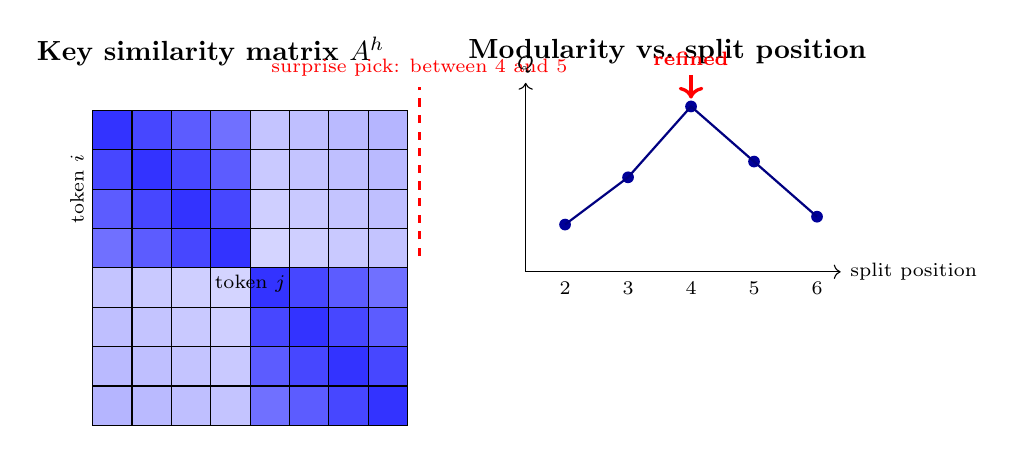
\begin{tikzpicture}[
  font=\footnotesize,
  cell/.style={draw, rectangle, minimum width=0.5cm, minimum height=0.5cm, inner sep=0pt},
  node distance=0.5cm,
]

% --- Left panel: similarity matrix as a heatmap ---
\begin{scope}[xshift=0cm, yshift=0cm]
  \node[font=\bfseries] at (2.0, 3.0) {Key similarity matrix $A^h$};

  % Generate an 8x8 grid with two block-diagonal communities at positions 1-3 and 5-8.
  % Color intensity ~ similarity. Within-cluster is darker.
  \foreach \i in {1,...,8} {
    \foreach \j in {1,...,8} {
      \pgfmathsetmacro{\val}{
        ifthenelse((\i<5 && \j<5) || (\i>4 && \j>4),
          80 - 8*abs(\i-\j),    % within-cluster
          15 + 2*abs(\i-\j))    % across-cluster
      }
      \pgfmathsetmacro{\colorval}{min(100, max(5, \val))}
      \node[cell, fill=blue!\colorval!white]
        at ({\j*0.5 + 0.25}, {2.5 - \i*0.5}) {};
    }
  }

  % Candidate boundary line at position 4-to-5 (surprise pick).
  \draw[red, very thick, dashed] (4.65, 0.4) -- (4.65, 2.55) node[above, font=\scriptsize] {surprise pick: between 4 and 5};

  % Axis labels.
  \node[font=\scriptsize] at (2.5, 0.05) {token $j$};
  \node[font=\scriptsize, rotate=90] at (0.3, 1.25) {token $i$};
\end{scope}

% --- Right panel: modularity score at each candidate split position ---
\begin{scope}[xshift=6.0cm, yshift=0.2cm]
  \node[font=\bfseries] at (1.8, 2.8) {Modularity vs.\ split position};

  % Axes
  \draw[->] (0, 0) -- (4.0, 0) node[right, font=\scriptsize] {split position};
  \draw[->] (0, 0) -- (0, 2.4) node[above, font=\scriptsize] {$Q$};

  % Data points: a peak at position 4 (correct boundary), lower at 3 and 5.
  \foreach \x/\y/\lbl in {0.5/0.6/2, 1.3/1.2/3, 2.1/2.1/4, 2.9/1.4/5, 3.7/0.7/6} {
    \node[circle, fill=blue!60!black, inner sep=1.5pt] at (\x, \y) {};
    \node[below, font=\scriptsize] at (\x, 0) {\lbl};
  }

  % Connect them.
  \draw[blue!50!black, thick]
    (0.5, 0.6) -- (1.3, 1.2) -- (2.1, 2.1) -- (2.9, 1.4) -- (3.7, 0.7);

  % Mark the chosen split with a red arrow.
  \draw[red, very thick, ->] (2.1, 2.5) -- (2.1, 2.2);
  \node[red, font=\scriptsize\bfseries, above] at (2.1, 2.5) {refined};
\end{scope}

\end{tikzpicture}

\caption{Refinement as a graph cut. Left: the key similarity matrix has two soft communities (positions 1--4 and 5--8) with a band of weak cross-cluster similarity in between. The surprise threshold marks position 4--5 as a candidate boundary. Right: modularity is evaluated at each candidate split position within a refinement window; the position that maximises $Q$ is the refined boundary.}
\label{fig:boundary-refinement}
\end{figure}

\paragraph{Why it helps and what it costs.}
The intuition is that surprise picks out the rough location of an event change but the precise location can sit one or two tokens to either side of the surprise spike. The refinement step lets the similarity structure of the keys speak. If $\alpha$ and $\beta$ are adjacent candidate boundaries, the algorithm searches positions strictly between them and picks the one whose induced split scores best under $f$. The complexity is $O(nm)$ where $n$ is the sequence length and $m$ is the chunk size used to process the sequence (Appendix C.1 of the paper); in practice $m$ is set so that the refinement cost is small compared with the cost of the attention itself. The paper reports modularity slightly outperforming conductance on the experimental tasks, but both improve over surprise alone.

\subsection{Two-stage memory retrieval}
\label{sec:method-retrieval}

Once events are stored, the question is which ones to bring back when the LLM generates the next token. EM-LLM's answer combines two retrieval signals, one based on content similarity and one based on temporal neighbourhood. Each transformer layer runs both independently.

\paragraph{Stage one: similarity buffer.}
For the current attention query, the system performs a $k$-nearest-neighbour lookup over stored events. The key used for the comparison is not the full event but a small set of \emph{representative tokens} per event, chosen as the most influential tokens within the event in the sense of \textcite{xiao2024infllm}. The top $k_s$ events by dot-product similarity to the query enter the similarity buffer. For small memories this lookup is exact; for memories large enough to spill to CPU or disk (the 10M-token regime in particular) the implementation uses an approximate $k$-NN library.

\paragraph{Stage two: contiguity buffer.}
When an event is retrieved by similarity, EM-LLM also enqueues its temporal neighbours, the events that originally fell within $\pm n$ positions in the source sequence (the paper uses $n = 1$ throughout). The contiguity buffer is a fixed-size queue of capacity $k_c$. When the queue fills, older or already-attended events are dequeued. This is the operational analogue of the contiguity effect from \cref{sec:episodic}: items studied close together in time should be available together at recall.

\begin{figure}[h]
\centering
% Two-stage retrieval. Each transformer layer runs both stages independently.
% Used in Chapter 3 (method) and referenced from Chapter 8 (walkthrough).

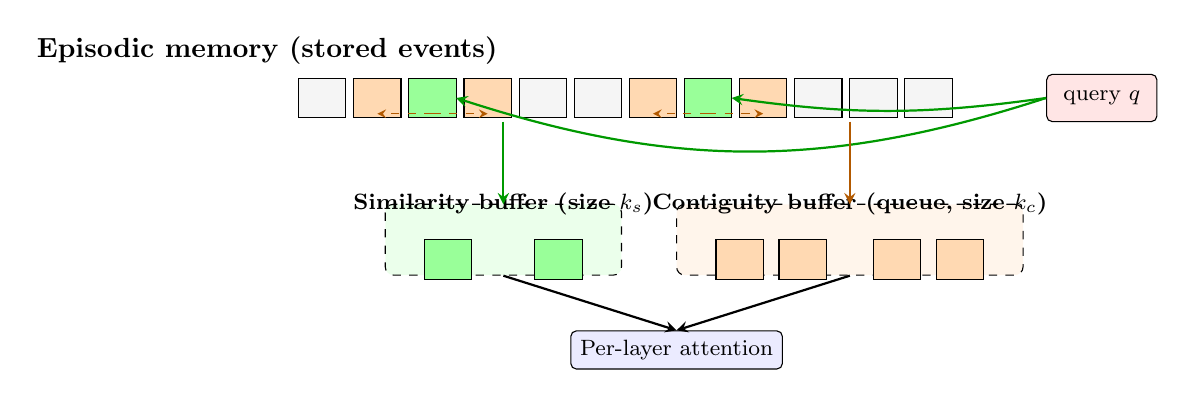
\begin{tikzpicture}[
  font=\footnotesize,
  event/.style={draw, rectangle, minimum width=0.6cm, minimum height=0.5cm, inner sep=1pt},
  query/.style={draw, rounded corners=2pt, fill=red!10, minimum width=1.4cm, minimum height=0.6cm},
  buffer/.style={draw, dashed, rounded corners=3pt, inner sep=6pt},
  arrow/.style={->, >=stealth, thick},
  faded/.style={fill=gray!8},
]

% Event store: a row of 12 stored events with two highlighted as top-k hits.
\node[font=\bfseries] at (0, 1.8) {Episodic memory (stored events)};
\foreach \i in {1,...,12} {
  \node[event, faded] (e\i) at (\i * 0.7, 1.2) {};
}
% Two top-similarity hits, dark green.
\node[event, fill=green!40] at (3 * 0.7, 1.2) {};
\node[event, fill=green!40] at (8 * 0.7, 1.2) {};
% Neighbours of the hits (enqueued into contiguity buffer), light orange.
\node[event, fill=orange!30] at (2 * 0.7, 1.2) {};
\node[event, fill=orange!30] at (4 * 0.7, 1.2) {};
\node[event, fill=orange!30] at (7 * 0.7, 1.2) {};
\node[event, fill=orange!30] at (9 * 0.7, 1.2) {};

% Query at the right.
\node[query] (q) at (10.6, 1.2) {query $q$};

% Similarity arrows (curved, green).
\draw[arrow, green!60!black] (q.west) to[bend left=18] (3 * 0.7 + 0.3, 1.2);
\draw[arrow, green!60!black] (q.west) to[bend left=8]  (8 * 0.7 + 0.3, 1.2);

% Contiguity arrows (curved, orange) from green hits to their neighbours.
\draw[->, >=stealth, dashed, orange!70!black] (3 * 0.7, 1.0) -- (2 * 0.7, 1.0);
\draw[->, >=stealth, dashed, orange!70!black] (3 * 0.7, 1.0) -- (4 * 0.7, 1.0);
\draw[->, >=stealth, dashed, orange!70!black] (8 * 0.7, 1.0) -- (7 * 0.7, 1.0);
\draw[->, >=stealth, dashed, orange!70!black] (8 * 0.7, 1.0) -- (9 * 0.7, 1.0);

% The two buffers below.
\node[buffer, fill=green!8, minimum width=3.0cm, minimum height=0.9cm] (simbuf) at (3.0, -0.6) {};
\node[font=\footnotesize\bfseries] at (3.0, -0.15) {Similarity buffer (size $k_s$)};
\node[event, fill=green!40] at (2.3, -0.85) {};
\node[event, fill=green!40] at (3.7, -0.85) {};

\node[buffer, fill=orange!8, minimum width=4.4cm, minimum height=0.9cm] (cbuf) at (7.4, -0.6) {};
\node[font=\footnotesize\bfseries] at (7.4, -0.15) {Contiguity buffer (queue, size $k_c$)};
\node[event, fill=orange!30] at (6.0, -0.85) {};
\node[event, fill=orange!30] at (6.8, -0.85) {};
\node[event, fill=orange!30] at (8.0, -0.85) {};
\node[event, fill=orange!30] at (8.8, -0.85) {};

% Arrows from the event store into the two buffers.
\draw[arrow, green!60!black] (3.0, 0.9) -- (3.0, -0.15);
\draw[arrow, orange!70!black] (7.4, 0.9) -- (7.4, -0.15);

% Final union arrow into attention.
\node[font=\footnotesize, draw, rounded corners=2pt, fill=blue!8, minimum width=2.4cm] (attn) at (5.2, -2.0) {Per-layer attention};
\draw[arrow] (simbuf.south) -- (attn.north);
\draw[arrow] (cbuf.south) -- (attn.north);

\end{tikzpicture}

\caption{Two-stage retrieval for one generation step. The similarity buffer picks the $k_s$ events whose representative tokens best match the current query under dot-product similarity (solid green arrows). The contiguity buffer enqueues the temporal neighbours of those events (dashed orange arrows). Both feed into the per-layer attention.}
\label{fig:two-stage-retrieval}
\end{figure}

\paragraph{Total context.}
The total number of retrieved events at each step is $k = k_s + k_c$. The paper expresses experimental settings in tokens rather than events, so configurations like ``4k local + 4k retrieved'' refer to maximum token budgets. The split between similarity and contiguity is controlled by the contiguity ratio $k_r = k_c / k$. The paper sweeps $k_r \in \{0.3, 0.5, 0.7\}$ and reports $k_r = 0.3$ as a robust default; the similarity buffer dominates by token count, with the contiguity buffer playing a smaller, supplementary role.

\paragraph{Per-layer independence.}
Every transformer layer carries out its own retrieval. This is one of the design choices that most clearly separates EM-LLM from prompt-level RAG. A RAG system attends to retrieved chunks once, at the input layer, and then every later layer reads transformed versions of the same retrieved content. EM-LLM lets different layers pull in different events from the same memory store. The paper argues (Section~4.1, Fig.~1) that this per-layer flexibility is the main source of its 30.5-point LongBench advantage over the NV-Embed-v2 RAG baseline.

\paragraph{Putting the pieces together.}
For each generated token, each layer attends to four regions in sequence: the 128 initial-token attention sinks, the contiguity buffer (events temporally adjacent to recently retrieved events), the similarity buffer (events most similar to the current query), and the local context window of recent tokens (working memory). Tokens outside these regions are invisible to the softmax at that step. Memory beyond the local window is not lost; it is just not loaded into attention until similarity or contiguity calls for it. \cref{sec:architecture} formalises this layout and walks through how RoPE and the patch into Hugging Face transformers actually carry it out at the code level.


\section{Architecture and hyperparameters}
\label{sec:architecture}

This chapter pins down what EM-LLM looks like as an operational object: the layout of the effective context, the positional encoding convention for retrieved tokens, the way the wrapper attaches to a Hugging Face model, and the hyperparameters a user actually sets at runtime.

\subsection{The three-part context}
\label{sec:three-part-context}

At every generation step, each transformer layer attends to a context that is a union of three groups (paper Fig.\ 3C). The groups are disjoint and the boundaries are explicit.

\paragraph{Initial tokens.}
The first 128 token positions are held fixed across the entire run. They are not segmented into events and they are not subject to eviction. Following \textcite{xiao2024attsinks}, these positions act as attention sinks: even after the rest of the long history has been swapped out to episodic memory, the softmax in each head can still concentrate mass on the sinks, which stabilises the attention distribution. The exact count of 128 is inherited from the InfLLM defaults and is not reported as sensitive in the EM-LLM ablations.

\paragraph{Local context.}
The local context holds the most recent tokens that fit inside the underlying LLM's training window (typically 4K). Within this window the model runs full softmax attention with no modification. This is the part of EM-LLM that behaves like an unaltered transformer, and it carries the analogy to working memory: a small, attention-controlled buffer that holds whatever is needed for the immediate task \cite{baddeley1992working,cowan2001focus}.

\begin{figure}[h]
\centering
% The four regions that make up the effective context at one generation step.
% Used in Chapter 4 (architecture) and referenced from Chapter 8 (walkthrough).

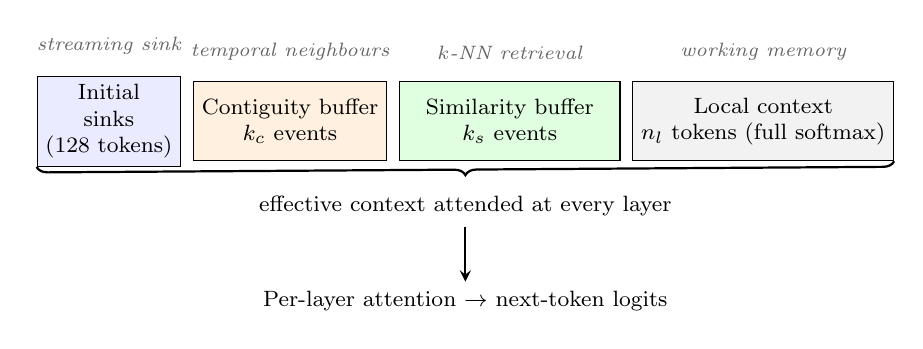
\begin{tikzpicture}[
  font=\footnotesize,
  region/.style={draw, minimum height=1.0cm, align=center, inner sep=3pt},
  sink/.style={region, fill=blue!8, minimum width=1.3cm},
  contig/.style={region, fill=orange!12, minimum width=2.2cm},
  sim/.style={region, fill=green!12, minimum width=2.8cm},
  local/.style={region, fill=gray!10, minimum width=3.0cm},
  arrow/.style={->, >=stealth, thick},
  label/.style={font=\scriptsize\itshape, text=black!60},
]

% The four regions, left to right.
\node[sink]   (sinks)  {Initial\\sinks\\(128 tokens)};
\node[contig] (cb) [right=0.15cm of sinks] {Contiguity buffer\\$k_c$ events};
\node[sim]    (sb) [right=0.15cm of cb]    {Similarity buffer\\$k_s$ events};
\node[local]  (lc) [right=0.15cm of sb]    {Local context\\$n_l$ tokens (full softmax)};

% Above-label: what cognitively-styled role each region plays.
\node[label, above=0.15cm of sinks] {streaming sink};
\node[label, above=0.15cm of cb]    {temporal neighbours};
\node[label, above=0.15cm of sb]    {$k$-NN retrieval};
\node[label, above=0.15cm of lc]    {working memory};

% Below brace and arrow indicating the LLM forward consumes the union.
\draw[decorate, decoration={brace, mirror, amplitude=4pt}, thick]
  (sinks.south west) -- (lc.south east)
  node[midway, below=8pt, font=\footnotesize] (brace) {effective context attended at every layer};

\node[below=0.7cm of brace, font=\footnotesize] (attn) {Per-layer attention $\rightarrow$ next-token logits};
\draw[arrow] (brace) -- (attn);

\end{tikzpicture}

\caption{The effective context at one generation step, in four regions. The local context behaves like an unmodified transformer window; the two retrieval buffers paginate the episodic store into the LLM's view; the initial-token sinks stabilise attention. Each layer re-runs retrieval, so different layers can attend to different events.}
\label{fig:context-layout}
\end{figure}

\paragraph{Evicted tokens (episodic memory).}
Everything older than the local context lives in the episodic store. These tokens are organised into events by the segmentation and refinement steps of \cref{sec:method}. The events are kept in a KV cache that can stay on GPU, spill to CPU, or be paged to disk depending on memory pressure (the \file{ContextManager} class, walked through in \cref{sec:walkthrough}). At each generation step, the similarity buffer and the contiguity buffer load a subset of these events back into the LLM's effective context for that step alone; events not retrieved are invisible to the softmax during that step but are not deleted.

The total effective context at one generation step is therefore the union of: initial tokens, contiguity buffer events, similarity buffer events, and local context tokens. The sizes of the two buffers are governed by the hyperparameters in \cref{sec:hparams}.

\subsection{Positional encoding for retrieved tokens}
\label{sec:rope-retrieved}

Retrieved events sit at original positions that can be millions of tokens deep. Asking the LLM to apply its native RoPE rotation at such positions is not a good plan: the positional embeddings the model was trained on never reached those values, and the predictable consequence is degraded attention quality even when the underlying tokens are sensible \cite{kazemnejad2024impact,su2024roformer}.

EM-LLM's response, following \textcite{xiao2024infllm}, is to assign retrieved tokens a fixed, in-distribution positional encoding rather than their true original positions. The choice mirrors the approach that \textcite{raffel2020exploring} used in T5, where retrieved content is treated as a separate, near-origin segment for the purpose of position-aware attention. Concretely, after a similarity or contiguity retrieval pulls an event back into the context, the retrieved tokens are placed at positions that the LLM has seen during training; the local context continues to use its native RoPE positions. This preserves the LLM's normal attention behaviour on retrieved content at the cost of not telling the LLM how far back in the original stream the retrieved tokens came from. That distance signal, the paper argues, is more usefully carried by the contiguity buffer.

\subsection{Wrapping a frozen LLM via \texttt{patch\_hf}}
\label{sec:patch-hf}

The whole pipeline operates as a runtime patch on a Hugging Face \texttt{transformers} model. The function \file{em\_llm.utils.patch\_hf.patch\_hf} replaces the attention-forward methods of the target model with EM-LLM's own implementation; it does not fork \file{transformers} and it does not require a model rewrite. The LLM weights are loaded normally, then the patch swaps in the EM-LLM context manager, the surprise-driven boundary detector, and the per-layer retrieval logic.

Five base models are supported in the released codebase, and each ships with a matching configuration template under \file{em-llm-model/benchmark/config/}: Mistral-7B-v0.2 \cite{jiang2023mistral}, LLaMA-2-7B \cite{touvron2023llama2}, LLaMA-3-8B and LLaMA-3.1-8B \cite{meta2024llama3}, and Phi-3 and Phi-3.5 \cite{abdin2024phi3}. The patch is architecture-aware in the limited sense that it knows the attention class name of each model; adding a new model requires extending that lookup but no other change to the EM-LLM core. The walkthrough in \cref{sec:walkthrough-patch-hf} traces the actual mechanics.

The current release supports batch size 1 only. This is a hard constraint asserted in \file{context\_manager.py}, not a guideline. It is the most visible operational limit of the codebase and the most likely thing to bite a reproducer who tries to use the wrapper for evaluation in parallel rather than running multiple jobs.

\subsection{Hyperparameters}
\label{sec:hparams}

\cref{tab:hparams} collects the runtime knobs a user typically adjusts, the symbol used in the paper, the role each one plays, the range explored in the paper's experiments, and the value the reproduction uses as a default. Where the paper and the implementation disagree on naming, both names are given.

\begin{table}[h]
\centering
\footnotesize
\begin{tabular}{>{\raggedright\arraybackslash}p{3.2cm}>{\raggedright\arraybackslash}p{5.2cm}>{\raggedright\arraybackslash}p{2.6cm}>{\raggedright\arraybackslash}p{2.2cm}}
  \toprule
  Symbol (paper) & Role & Range tested & Default \\
  \midrule
  $\gamma$ & Surprise threshold scale in \cref{eq:threshold}; larger $\gamma$ means fewer boundaries & 1.0, 1.5, 2.0, 2.5, 3.0, 3.5 & $1.0$ \\
  $\tau$ & Trailing window length for $\mu$ and $\sigma$ in \cref{eq:threshold} & implementation default & per config \\
  $k$ & Total retrieved-event budget per layer, in tokens & $4\text{K}, 8\text{K}$ in reported runs & $4\text{K}{+}4\text{K}$ \\
  $k_r = k_c / k$ & Fraction of $k$ devoted to the contiguity buffer & $\{0.3, 0.5, 0.7\}$ & $0.3$ \\
  $n$ & Neighbour radius for the contiguity buffer, in events & $1$ throughout the paper & $1$ \\
  $m$ & Chunk size for the boundary refinement loop & implementation default & per config \\
  refinement metric & Modularity vs.\ conductance (\cref{eq:modularity,eq:conductance}) & both reported & modularity \\
  \texttt{\seqsplit{max\_block\_size}} & Maximum tokens per stored event & not a paper hyperparameter & per config \\
  \texttt{\seqsplit{min\_free\_cpu\_memory}} & Memory headroom before CPU offload triggers & not a paper hyperparameter & 8 GB on RTX 3090 \\
  \texttt{\seqsplit{disk\_offload\_threshold}} & Token count above which events page to disk & not a paper hyperparameter & 200{,}000 on RTX 3090 \\
  \texttt{\seqsplit{vector\_offload\_threshold}} & Token count above which event reps page to CPU & not a paper hyperparameter & 30{,}000 on RTX 3090 \\
  \bottomrule
\end{tabular}
\caption{Runtime hyperparameters of EM-LLM. The top block lists parameters from the paper itself; the bottom block lists implementation-only knobs that govern offload behaviour and are tuned per hardware setup in \file{docs/hardware\_adaptations.md}.}
\label{tab:hparams}
\end{table}

The most consequential choice for a reproducer is the local-plus-retrieved budget, written in the configs as ``4k+4k'' or ``4k+2k''. The first number is the size of the local window, the second the size of the retrieved buffer, both in tokens. The paper's main results table (Table~1) uses 4k+2k for Mistral-v0.2 and 4k+4k for the LLaMA-3 family, matching the InfLLM baseline budgets so comparisons are like-for-like. The Phi family uses 1k+3k, again matching the InfLLM setting for those models.

The offload thresholds in the lower block of \cref{tab:hparams} do not appear in the paper but matter for any run that approaches the 1M-plus token regime on commodity GPUs. They are documented separately in \file{docs/hardware\_adaptations.md} and discussed in \cref{sec:repro-pipeline}.


\section{Evaluation and results}
\label{sec:evaluation}

The paper backs the architecture with three families of experiments: long-context accuracy on standard benchmarks (\cref{sec:eval-longcontext}), agreement with human-annotated event boundaries on podcast transcripts (\cref{sec:human-alignment}), and graph-theoretic measurements of segmentation quality on PG-19 (\cref{sec:eval-segmentation}). The ablation table at the end (\cref{sec:eval-ablations}) breaks each component out so that a reproducer can attribute the gains.

\subsection{Benchmarks and baselines}
\label{sec:eval-benchmarks}

\paragraph{LongBench.}
LongBench \cite{bai2023longbench} is the main accuracy benchmark in the paper. The reported runs use six task groups: single-document QA (NarrativeQA, Qasper, MultiFieldQA), multi-document QA (HotpotQA, 2WikiMultihopQA, MuSiQue), summarisation (GovReport, QMSum, MultiNews), few-shot learning (TREC, TriviaQA, SAMSum), retrieval (PassageRetrieval, PassageCount), and coding (LCC, RepoBench-P). Each task contributes one score; the per-group score in Table~1 of the paper is the mean over the tasks in that group.

\paragraph{$\infty$-Bench.}
$\infty$-Bench \cite{zhang2024infbench} pushes context length into the hundred-thousand-token range. The reported runs use Code.Debug (C.D), Math.Find (M.F), Multi-Choice (MC), Retrieve.KV (R.KV), Retrieve.PassKey (R.P), and Retrieve.Number (R.N). The retrieval-style tasks (R.KV, R.P, R.N) are where EM-LLM has the largest margins, which is consistent with the paper's claim that the per-layer retrieval is precisely what helps.

\paragraph{Extended passkey retrieval.}
The 10M-token scalability claim comes from an extension of $\infty$-Bench's PassKey task. Baseline data for the long-context curve in Fig.~1 is taken from \textcite{ding2024longrope}, which lets EM-LLM be plotted alongside YaRN, LongRoPE-2048k, and the original PassKey settings on a common axis.

\paragraph{Baselines.}
Three baselines run head-to-head with EM-LLM: InfLLM \cite{xiao2024infllm} as the previous SOTA in group-based $k$-NN retrieval, RAG built on NV-Embed-v2 \cite{lee2024nvembed} as the strongest current embedding-retriever, and full-context inference with the base LLM as a brute-force upper bound (which only runs where the context fits in memory). The paper also runs a custom surprise-based RAG ablation that uses EM-LLM's surprise signal to pick chunks for a single-step retrieval, which isolates the contribution of EM-LLM's layer-wise mechanism from the contribution of surprise itself.

\paragraph{Metrics.}
LongBench scores combine F1 (QA, retrieval), ROUGE-L (summarisation), accuracy (few-shot, coding), and exact match where appropriate. $\infty$-Bench uses task-native accuracy. Segmentation-quality experiments use the three graph-theoretic measures from \cref{sec:method-refinement}: modularity, conductance, and the intra/inter-similarity ratio (I/IS) defined in Eq.\ 5 of the paper. The human-alignment experiment uses the Wasserstein distance between each method's boundary positions and the human-annotated boundary positions.

\subsection{Long-context accuracy}
\label{sec:eval-longcontext}

\cref{tab:headline} reproduces the most salient cells of paper Table~1. The variant labels are S (surprise only), SM (surprise + modularity refinement), SC (surprise + conductance refinement), and SM+C (SM with contiguity buffer added). The numbers come straight from the paper; this companion does not re-run the benchmarks.

\begin{table}[h]
\centering
\footnotesize
\begin{tabular}{lllcccc}
  \toprule
  Base LLM & Method & Budget & LongBench avg.\ & Retrieval task & $\infty$-Bench R.KV & R.P \\
  \midrule
  Mistral-v0.2 & InfLLM & 4k+2k & 41.9 & 64.0 & 95.6 & 100 \\
  Mistral-v0.2 & EM-LLM (SM+C) & 4k+2k & \textbf{43.7} & \textbf{84.1} & \textbf{99.0} & 100 \\
  \midrule
  LLaMA-3-8B & InfLLM & 4k+4k & 47.0 & 84.0 & 5.0 & 100 \\
  LLaMA-3-8B & EM-LLM (S) & 4k+4k & \textbf{47.2} & \textbf{87.5} & 4.2 & 100 \\
  \midrule
  LLaMA-3.1-8B & InfLLM & 4k+4k & 51.1 & 97.0 & 81.0 & 100 \\
  LLaMA-3.1-8B & EM-LLM (SM) & 4k+4k & \textbf{51.3} & \textbf{98.5} & \textbf{90.2} & 100 \\
  \bottomrule
\end{tabular}
\caption{Selected rows from paper Table~1. LongBench avg.\ is the mean over the six task groups. ``Budget'' is local tokens plus retrieved tokens. Bold entries are where EM-LLM beats InfLLM at the same budget.}
\label{tab:headline}
\end{table}

The pattern is consistent. EM-LLM almost always edges the InfLLM baseline on aggregate, with the biggest jumps on retrieval and QA. The single negative on this slice is LLaMA-3-8B's $\infty$-Bench Retrieve.KV, where surprise-only segmentation slightly trails fixed-size segmentation (4.2 vs.\ 5.0); both scores are low in absolute terms, indicating the task is failing for both methods rather than a real loss in EM-LLM. The paper notes this in Appendix~A.1 and recommends the SM+C variant when Retrieve.KV matters.

\paragraph{Against RAG and full-context.}
On LLaMA-3.1-8B and LongBench, EM-LLM scores 51.58\% in the surprise-only setting, RAG with NV-Embed-v2 scores 36.44\%, and the full-context baseline scores 39.3\% (Fig.~1 of the paper). The 30.5-point gap over RAG is the headline of the paper's introduction and is consistent with the per-layer retrieval argument made in \cref{sec:method-retrieval}: RAG retrieves once at the input layer, EM-LLM retrieves at every layer independently.

\paragraph{Scaling to 10M tokens.}
Fig.~1 (bottom) of the paper plots passkey-retrieval accuracy against sequence length for EM-LLM, YaRN-extended Mistral, LongLoRA + CodeLLaMA, and LongRoPE-2048k. EM-LLM holds 100\% accuracy at 10.2M tokens, two orders of magnitude past the practical ceiling of full-context Mistral. The complexity expression behind this is $O(n(n_l + n_r) + n(n - n_l)/m \cdot b)$, where $n$ is the sequence length, $n_l$ the local window size, $n_r$ the retrieved budget, $m$ the refinement chunk size, and $b$ the refinement cost per chunk (Appendix C.1). The dominant term is sublinear in $n$ once the local window and the retrieved budget are fixed.

\subsection{Agreement with human event segmentation}
\label{sec:human-alignment}

The second experiment evaluates segmentation quality directly rather than through downstream task accuracy. The data are three human-annotated podcast transcripts from \textcite{kumar2023neural}, with ground-truth event boundaries provided by listeners.

The paper compares six segmentation methods on these transcripts: F (fixed-size), FM (fixed + modularity refinement), FC (fixed + conductance refinement), S (surprise only), SM (surprise + modularity), and SC (surprise + conductance). For each method, the per-layer modularity, conductance, and I/IS of the induced segmentation are computed and compared with the same metrics on the human-annotated segmentation.

Two patterns come out of Fig.~4 of the paper. First, surprise-based methods (S, SM, SC) match human segmentation more closely than fixed-size methods (F, FM, FC), and InfLLM's fixed-size method (F) is the only one whose modularity score sits below random. Second, refinement adds further improvement on top of surprise: SM and SC each push modularity higher than S alone. The Wasserstein distance between each method's boundary positions and the human positions follows the same ranking: S, SM, and SC are closest to humans, with SM the closest of the three on average.

This is the result most directly relevant to readers who care whether ``LLM surprise looks like human surprise''. The answer the paper supports is qualified yes: not pixel-perfect agreement, but the same ranking of methods on the same task.

\subsection{Segmentation quality on PG-19}
\label{sec:eval-segmentation}

Table~2 of the paper reports the same three graph metrics on the PG-19 long-text corpus, this time without human ground truth. The numbers are differences from random segmentation, so positive modularity and I/IS values, and negative conductance values, indicate gains over chance.

On every base LLM tested (Mistral-7B, LLaMA-2-7B, LLaMA-3-8B), the ranking is consistent. Fixed-size segmentation (F) is essentially indistinguishable from random by modularity and I/IS, and worse than random by conductance. Surprise-based methods are well above random on all three metrics. Adding refinement on top of surprise (SM, SC) gives a further boost, with SM (modularity refinement) doing the best on the modularity score, as one would expect from a method that explicitly optimises modularity. The takeaway is that surprise picks rough event locations and refinement sharpens them, with each step measurable in graph-theoretic terms.

\subsection{Ablations}
\label{sec:eval-ablations}

The ablation analysis (paper Section~4.4, Tables~3--7 in the appendix) is the part most useful for setting expectations on a reproduction. Three high-level findings:
\begin{itemize}
  \item \textbf{Refinement} alone (S vs.\ SM, SC) improves performance in roughly 60\% of LongBench and $\infty$-Bench tasks. The improvement is largest on QA and retrieval tasks, where coherent event boundaries help the $k$-NN find the right block.
  \item \textbf{Contiguity buffer} alone (S vs.\ S+C, SM vs.\ SM+C) improves performance in roughly 44\% of tasks. The improvement is concentrated on tasks where temporal order matters: multi-document QA in particular.
  \item \textbf{The two are complementary}, not redundant. The best variant for a given task is usually SM+C, but the paper does not claim a universal winner; some tasks favour S, others SM or SC.
\end{itemize}
The paper also reports a sweep over the contiguity ratio $k_r = k_c / k$ at $\{0.3, 0.5, 0.7\}$ (Fig.~13 of the appendix). The result is that contiguity buffers as large as or smaller than the similarity buffer ($k_r \le 0.5$) work best, with $k_r = 0.3$ the most common winner. The similarity buffer carries most of the load; the contiguity buffer is a useful supplement, not a replacement.


\section{Limitations and open questions}
\label{sec:limitations}

This chapter pulls together the limitations the paper itself acknowledges, the future directions it points to, and the questions a reproducer should keep in mind as they run the experiments in this repository. The reproduction's own answers to these questions, when they come, belong in \file{docs/differences\_from\_paper.md} rather than in this companion.

\subsection{Acknowledged limitations}

\paragraph{The clustering metric is not universal.}
The paper uses modularity and conductance, and reports modularity as the better default. It does not claim either metric is optimal across all networks or all tasks. \textcite{fortunato2010community} and the broader community-detection literature show that the relative performance of community metrics depends on the underlying graph structure, and the paper points to this explicitly in Section~5. A reproducer who finds modularity underperforms on a particular task should not assume the implementation is broken; it could be a domain mismatch the paper does not cover.

\paragraph{Hyperparameter sensitivity is only lightly explored.}
The paper sweeps $\gamma$ at six values, the contiguity ratio $k_r$ at three, and the refinement metric at two. The chunk size $m$, the trailing window length $\tau$, the neighbour radius $n$, and the offload thresholds are mostly held at implementation defaults. The combined space is small enough that nothing obvious is missing, but it also means a thorough reproducer has room to find sensitivities the original work did not expose.

\paragraph{Task-dependent component value.}
Section~4.4 of the paper observes that refinement improves 60\% of tasks and contiguity 44\%, but the best variant for a given task is not always SM+C. Some tasks favour S alone, some SM, some SC, some S+C. The paper does not propose a model for predicting which variant wins on which task; choosing per-task is left to the practitioner.

\paragraph{Memory overhead at 1M-plus tokens.}
The paper reports the 10M-token passkey result without dwelling on the engineering cost. In practice, holding 10M tokens of KV pairs plus event representatives is well past GPU memory on commodity hardware, and the implementation relies on CPU and disk offload via \texttt{min\_free\_cpu\_memory}, \texttt{disk\_offload\_threshold}, and \texttt{vector\_offload\_threshold} (\cref{sec:hparams}). Those knobs are not paper hyperparameters; they are an artefact of running long sequences on real machines. This reproduction handles them through \file{docs/hardware\_adaptations.md} and the configs under \file{reproduction/configs/}.

\paragraph{Batch size one.}
The released implementation supports batch size 1 only. This is asserted as a hard constraint in \file{em\_llm/attention/context\_manager.py} and is not lifted by any configuration flag in the current codebase. A reproducer who wants to evaluate the wrapper at higher throughput is forced into multiple processes rather than larger batches.

\subsection{Author-stated future directions}

\paragraph{Per-layer segmentation.}
EM-LLM currently segments tokens once, into one canonical set of events, and then retrieves from that set at every layer. The paper proposes (Section~5) extending segmentation to operate independently at each transformer layer, producing a hierarchical event structure. This would parallel the multi-scale event hierarchy observed in human cortex \cite{baldassano2017discovering} and the per-layer roles already observed in induction heads.

\paragraph{Imagination and future thinking.}
The authors point to model-based reinforcement learning and continual learning as natural beneficiaries of an episodic memory built on top of an LLM. The argument is that an LLM with explicit access to its own event history can simulate variants of past episodes, in effect imagining alternative futures, and that this kind of replay has been productive in the cognitive-science literature on memory \cite{spens2024construction}.

\paragraph{Advanced clustering and change-point detection.}
The surprise-based boundary rule in EM-LLM has a close formal relative in Bayesian online change-point detection \cite{adams2007bayesian}. The paper notes that more sophisticated change-point methods could replace the threshold-based detector, particularly for streaming data where the trailing-window statistics break down. This is one of the more concrete suggestions in Section~5 and is a candidate for the \file{extensions/} directory of this reproduction.

\paragraph{Multi-modal buffers.}
Following Baddeley's multi-component model of working memory, the authors suggest adding modality-specific buffers (visual, auditory) alongside the current text-only similarity and contiguity buffers. The cognitive analogy is straightforward; the engineering requires a multi-modal base model rather than the text-only LLMs the current paper uses.

\paragraph{Validation against human memory biases.}
The paper measures alignment with human event boundaries (\cref{sec:human-alignment}). It does not measure whether EM-LLM exhibits the recency, primacy, or asymmetry effects observed in human free recall. The authors propose running the same probes used in human memory studies against EM-LLM and comparing the resulting curves.

\subsection{Open questions for a reproducer}

The list below is shorter than the author-stated one and is what the reproducer in this repository specifically wants answered as the runs come in. It is not a contribution claim; it is a checklist.

\begin{itemize}
  \item Does the contiguity buffer help on multi-document QA more than it hurts on single-document QA, in our reproduction's runs, by the same margin as in the paper?
  \item At $k_r = 0.3$, what fraction of similarity-buffer events also appear in the contiguity buffer? A high overlap would suggest the two buffers are partly redundant; the paper does not report this.
  \item How sensitive is the 10M-token passkey result to the disk offload threshold? The paper does not vary the offload regime; the reproduction will.
  \item On Phi-3 and Phi-3.5, does the smaller base model exhibit a different optimal $\gamma$ than the LLaMA-3 family? The paper recommends $\gamma = 1.0$ across models but the Phi rows have weaker absolute scores.
  \item Does the modularity-vs-conductance preference depend on the genre of the input (news vs.\ legal vs.\ code)? The paper's PG-19 experiments mix fiction and non-fiction without breaking out the split.
\end{itemize}

These questions belong to this reproduction, not to the paper, and should be folded into \file{docs/differences\_from\_paper.md} as the runs produce evidence.


\printbibliography

\end{document}
